\documentclass[twoside]{article}

\usepackage{lipsum}
\usepackage[none]{hyphenat} 

\usepackage[sc]{mathpazo} 
\usepackage[T1]{fontenc} 
\linespread{1.05}
\usepackage{microtype}

\usepackage[hmarginratio=1:1,top=32mm,columnsep=20pt]{geometry}
\usepackage{multicol} 
\usepackage[hang, small,labelfont=bf,up,textfont=it,up]{caption} 
\usepackage{booktabs} 
\usepackage{float} 
\usepackage[hidelinks]{hyperref} 
\usepackage[usenames]{color}

\usepackage{lettrine} 
\usepackage{paralist}

\usepackage{abstract} 
\renewcommand{\abstractnamefont}{\normalfont\bfseries}
\renewcommand{\abstracttextfont}{\normalfont\small\itshape} 

\usepackage{titlesec} 
\renewcommand\thesection{\Roman{section}} 
\renewcommand\thesubsection{\Roman{subsection}} 
\titleformat{\section}[block]{\large\scshape\centering}{\thesection.}{1em}{} 
\titleformat{\subsection}[block]{\large}{\thesubsection.}{1em}{}

\usepackage{fancyhdr} 
\pagestyle{fancy} 
\fancyhead{} 
\fancyfoot{}

\fancyhead[C]{ Simulaci\'on $\bullet$ Eventos Discretos $\bullet$ Overloaded Harbor}
\fancyfoot[RO,LE]{\thepage}

\title{\vspace{-15mm}\fontsize{20pt}{10pt}\selectfont\textbf{Proyecto Eventos Discretos}}

\author{
\large
\textbf{\large Overloaded Harbor} \\[1.5cm]
\textsc{Alejandro Campos. C-411}\\\\[2mm]
\normalsize Facultad de Matem\'atica y Computaci\'on \\
\normalsize Universidad de la Habana \\
\normalsize 2021 \\[2cm]
\vspace{-5mm}
}
\date{}


\usepackage{graphicx}
\begin{document}

\maketitle

\thispagestyle{fancy} 

\section{Introducci\'on}

La simulaci\'on por eventos discretos es una t\'ecnica de modelado din\'amico de sistemas. Esta se caracteriza por un control en la variable del tiempo que permite avanzar a este a intervalos variables, en funci\'on de la planificaci\'on de ocurrencia de tales eventos a un tiempo futuro. Un requisito para aplicar esta t\'ecnica es que las variables que definen el sistema no cambien su comportamiento durante el intervalo simulado.

El problema de eventos discretos seleccionado para su resoluci\'on es Overloaded Harbor, cuya orden se detalla a continuaci\'on:\\

En un puerto de supertanqueros que cuenta con 3 muelles y un remolcador
para la descarga de estos barcos de manera simult\'anea se desea conocer el tiempo
promedio de espera de los barcos para ser cargados en el puerto.

El puerto cuenta con un bote remolcador disponible para asistir a los tanqueros.
Los tanqueros de cualquier tama\~no necesitan de un remolcador para
aproximarse al muelle desde el puerto y para dejar el muelle de vuelta al puerto.

El tiempo de intervalo de arribo de cada barco distribuye mediante una funci\'on exponencial con $\lambda$ = 8 horas. Existen tres tama\~nos distintos de tanqueros:
peque\~no, mediano y grande, la probabilidad correspondiente al tama\~no de cada
tanquero se describe en la tabla siguiente. El tiempo de carga de cada tanquero
depende de su tama\~no y los par\'ametros de distribuci\'on normal que lo representa
tambi\'en se describen en la tabla siguiente.\\

\begin{tabular}{c c c}
Tama\~no & Probabilidad de Arribo & Tiempo de Carga \\ \hline
Peque\~no & $0.25$ & $\mu = 9, \sigma^2 = 1$ \\
Mediano & $0.25$ & $\mu = 12, \sigma^2 = 2$ \\
Grande & $0.5$  & $\mu = 18, \sigma^2 = 3$ \\\\
\end{tabular}

De manera general, cuando un tanquero llega al puerto, espera en una cola
(virtual) hasta que exista un muelle vac\'io y que un remolcador est\'e disponible
para atenderle. Cuando el remolcador est\'a disponible lo asiste para que pueda
comenzar su carga, este proceso demora un tiempo que distribuye exponencial
con $\lambda$ = 2 horas. El proceso de carga comienza inmediatamente despu\'es de que
el barco llega al muelle. Una vez terminado este proceso es necesaria la asistencia
del remolcador (esperando hasta que est\'e disponible) para llevarlo de vuelta al
puerto, el tiempo de esta operaci\'on distribuye de manera exponencial con $\lambda$ = 1
hora. El traslado entre el puerto y un muelle por el remolcador sin tanquero
distribuye exponencial con $\lambda$ = 15 minutos.

Cuando el remolcador termina la operaci\'on de aproximar un tanquero al
muelle, entonces lleva al puerto al primer barco que esperaba por salir, en caso de
que no exista barco por salir y alg\'un muelle est\'e vac\'io, entonces el remolcador se
dirige hacia el puerto para llevar al primer barco en espera hacia el muelle vac\'io;
en caso de que no espere ning\'un barco, entonces el remolcador esperar\'a por alg\'un barco en un muelle para llevarlo al puerto. Cuando el remolcador termina
la operaci\'on de llevar alg\'un barco al puerto, este inmediatamente lleva al primer
barco esperando hacia el muelle vac\'io. En caso de que no haya barcos en los
muelles, ni barcos en espera para ir al muelle, entonces el remolcador se queda
en el puerto esperando por alg\'un barco para llevar a un muelle.

Simule completamente el funcionamiento del puerto. Determine el tiempo
promedio de espera en los muelles. \\\\

El objetivo de este informe es explicar el m\'etodo de resoluci\'on utilizado para resolver el problema anterior. Adem\'as explicaremos los detalles de implementaci\'on y ejecuci\'on de la aplicaci\'on, no sin antes abordar el modelo de eventos discretos utilizado y c\'omo se adapt\'o a este problema en particular. Por \'ultimo, haremos un an\'alisis de los resultados obtenidos a partir de la ejecuci\'on de las simulaciones del problema.\\\\

\section{Ideas principales para la soluci\'on del problema}
Para tratar este problema se siguieron las indicaciones de conferencia y del libro "Temas de simulaci\'on", cap\'itulo 3. Estos indican, en forma de resumen, que los elementos b\'asicos de una simulaci\'on basada en eventos discretos son las variables y los eventos. Luego cuando ocurra un evento los valores de las variables se actualizan y se genera el tiempo de ocurrencia del pr\'oximo evento. Posteriormente, se selecciona para ejecutar el evento cuyo tiempo sea menor.\\

En el caso de este problema, cuando un tanquero arriba al puerto se genera el tiempo del pr\'oximo arribo y se inserta en la lista de espera para ser movido a un muelle. Esta lista est\'a ordenada por el tiempo en que el tanquero ejecutar\'a su pr\'oximo evento, el siguiente evento a ejecutar ser\'a aquel cuyo tiempo sea menor y se pueda ejecutar seg\'un las condiciones del problema, ya que cada tanquero para moverse debe esperar a que el remolcador est\'e disponible, y que haya alg\'un muelle vac\'io, en caso de que el tanquero est\'e en el puerto. La forma de escoger el siguiente evento a procesar evita que un barco espere m\'as del tiempo que deber\'ia y evita, adem\'as, que un barco se quede esperando eternamente. Una vez que se pueda trasladar el barco hacia un muelle, se genera el tiempo del pr\'oximo evento, que ser\'ia la llegada del tanquero al muelle y el comienzo de la carga. De esta forma cada evento determina el tiempo del siguiente hasta que el tanquero abandona la simulaci\'on, guardando el tiempo de estancia desde su llegada hasta su partida antes de salir. Se tienen entonces los siguientes eventos a simular:
\begin{enumerate}
\item Llegada de un tanquero al puerto.
\item Traslado de un tanquero a un muelle si hay alguno disponible y el remolcador no est\'a ocupado.
\item Llegada de un tanquero al muelle e inicio de la carga.
\item Momento en que un tanquero termin\'o de cargar y est\'a listo para regresar al puerto cuando el remolcador est\'e disponible.
\item Traslado de un tanquero del muelle al puerto.
\item Llegada del tanquero al puerto y partida de este.
\end{enumerate}

Podemos mencionar, adem\'as, como evento adicional pero no correspondiente a los tanqueros, el movimiento del remolcador vac\'io hacia o desde los muelles en caso de que no hayan barcos esperando en el lugar donde se encuentra.\\

Por otro lado, debemos tener en cuenta a lo largo de la simulaci\'on: el tiempo general de esta, el tiempo de arribo y de partida de cada tanquero y el tiempo del pr\'oximo evento del mismo, constituyendo estas nuestras variables de tiempo. Las variables de estado, que describen el estado del puerto en el tiempo $t$, ser\'ian la localizaci\'on del remolcador (en el puerto, en el muelle o en movimiento) y la cantidad de muelles libres. Por \'ultimo, la cantidad de arribos y la lista de los tiempos que los tanqueros han estado en el puerto son nuestras variables contadoras.

Las variables anteriores constituyen la base de la simulaci\'on implementada, su uso concreto en el c\'odigo se ver\'a con mejor detalle en la secci\'on IV del presente informe.\\\\


\section{Modelo de Simulaci\'on de Eventos Discretos}
Para simular el problema se us\'o como base el modelo de eventos discretos de $n$ servidores en paralelo, o sea, cuando llega un cliente, si hay un servidor vac\'io se atiende a este, si todos est\'an llenos, se pone en la cola a esperar que uno se vac\'ie. En este problema los clientes ser\'ian los tanqueros y los servidores los muelles.

En el caso de este problema los clientes deben ser desplazados, por orden de llegada, a los servidores. Esta operaci\'on debe realizarse de uno en uno, puesto que solo se cuenta con un remolcador. Los clientes son atendidos por los servidores y posteriormente deben ser trasladados, tambi\'en de uno en uno, hacia la salida. Solo puede existir a lo sumo un cliente desplaz\'andose en el mismo intervalo de tiempo. El orden en que son desplazados a la salida depende del tiempo que demoren en llegar al servidor y lo que tarde el servidor en atenderlos (cargando el tanquero).  

La estancia de cada cliente en el sistema se calcula como la diferenca entre el tiempo de salida y el de llegada. Una vez concluida la simulaci\'on, la media del tiempo de todos los barcos ser\'ia la suma de sus tiempos dividido entre la cantidad de clientes que atendi\'o el sistema.\\\\

\section{Detalles de implementaci\'on}
La implementaci\'on de la simulaci\'on del problema en cuesti\'on se basa en las ideas anteriores. El c\'odigo est\'a suficientemente comentado como para entender la funcionalidad de cada uno de los m\'etodos y variables principales. No obstante explicamos en esta secci\'on, a muy groso modo, algunos detalles de implementaci\'on.

Tenemos dos clases principales: \textit{Tanker} y \textit{Harbor}. En la primera est\'an las propiedades correspondientes a los tanqueros, y toda la l\'ogica que corresponde a estos. Cada instancia de esta clase contiene el n\'umero de identificaci\'on de cada tanquero, el tiempo de llegada y de partida; adem\'as del tiempo \textit{current\_time} en que se ejecutar\'a el evento \textit{Event} asociado a cada barco, los cuales se modifican cada vez que se ejecuta un evento, pues en la ejecuci\'on del evento $i$ se conoce el siguiente evento $i+1$ a ejecutar y el tiempo de este. 

La clase \textit{Harbor} es la clase principal de la simulaci\'on, en esta se encuentran implementados cada uno de los eventos antes descritos. Para crear una instancia de esta clase debemos pasarle como par\'ametro el tiempo l\'imite de la simulaci\'on, este es el tiempo a partir del cual ya no entrar\'a ning\'un tanquero al puerto, pero la simulaci\'on continuar\'a hasta atender todos los tanqueros que quedan pendientes en el sistema. El n\'umero de muelles puede pasarse tambi\'en como par\'ametro a esta clase, de no pasarlo toma por defecto $3$ muelles. En esta clase se crea la lista \textit{pending\_tankers} que constituye la cola virtual de los tanqueros, la cual se mantiene ordenada durante toda la ejecuci\'on de la simulaci\'on, atendiendo al tiempo del pr\'oximo evento a ejecutar por los tanqueros. Mediante el m\'etodo \textit{run\_simulation} se desarrolla la simulaci\'on llamando al pr\'oximo evento m\'as cercano en el tiempo que pueda ejecutarse seg\'un la disponibilidad del remolcador y de los muelles.

El archivo \texttt{utils/utils.py} contiene los m\'etodos necesarios para generar los tiempos de cada evento. En este se encuentran los m\'etodos de generaci\'on de variables aleatorias con distribuci\'on exponencial con par\'ametro $\lambda$ y distribuci\'on normal con par\'ametros $\mu$ y $\sigma^2$.

Finalmente, en el archivo \texttt{main.py} se crea la instancia de la clase \textit{Harbor} seg\'un los par\'ametros que ingrese el usuario, y se ejecuta la simulaci\'on. En la siguiente secci\'on se describe mejor este proceso.

\section{Ejecuci\'on de la aplicaci\'on}
Para ejecutar la aplicaci\'on es necesario que el usuario tenga instalado python versi\'on $3.0$ o superior. Luego en la ubicaci\'on del proyecto debe abrir una consola y escribir \texttt{python main.py} y seguir los pasos que se indican.

La aplicaci\'on pedir\'a al usuario que ingrese el tiempo en horas a partir del cual ya no entrar\'a ning\'un barco en el puerto, no obstante, como ya se ha dicho, la simulaci\'on continuar\'a hasta atender a todos los barcos que a\'un est\'an dentro del sistema. Por lo que, potencialmente, la simulaci\'on durar\'a mucho m\'as que lo que indica este tiempo.

Despu\'es de ingresar este n\'umero se le pedir\'a al usuario que ingrese el n\'umero de muelles con que desea que la simulaci\'on se ejecute, de no entrar ning\'un n\'umero se asume por defecto $3$ muelles. Por \'ultimo, se pide el n\'umero de simulaciones que se realizar\'an con los par\'ametros antes solicitados, si no entra ning\'un n\'unmero se realizar\'a solo una simulaci\'on. En caso de que ingrese alg\'un dato inv\'alido, la aplicaci\'on lo notificar\'a y el usuario deber\'a ingresar los par\'ametros nuevamente.

Una vez concluida la o las simulaciones, se muestran el tiempo total, el n\'umero de barcos atendidos en ese tiempo y la media de  la estancia de los barcos en el puerto. El usuario podr\'a repetir el proceso presionando la tecla enter o salir escribiendo el comando \texttt{exit} en consola.\\\\

\section{Consideraciones obtenidas a partir de la ejecuci\'on de las simulaciones del problema}
Si el usuario realiza $10$ o m\'as simulaciones con los datos constantes, se muestran dos gr\'aficas que representan el comportamiento del tiempo de simulaci\'on y de la media de la estancia de los tanqueros, seg\'un los barcos que se atendieron.

A partir de realizar 30 simulaciones permitiendo la entrada de tanqueros hasta $5$ horas y con 3 muelles se obtuvieron los siguientes resultados:\\

\begin{figure}[h]

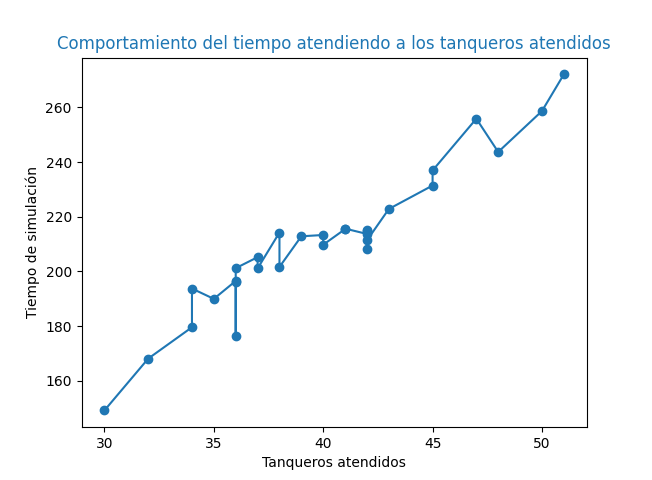
\includegraphics[scale = 0.39]{img/Figure_1.png}
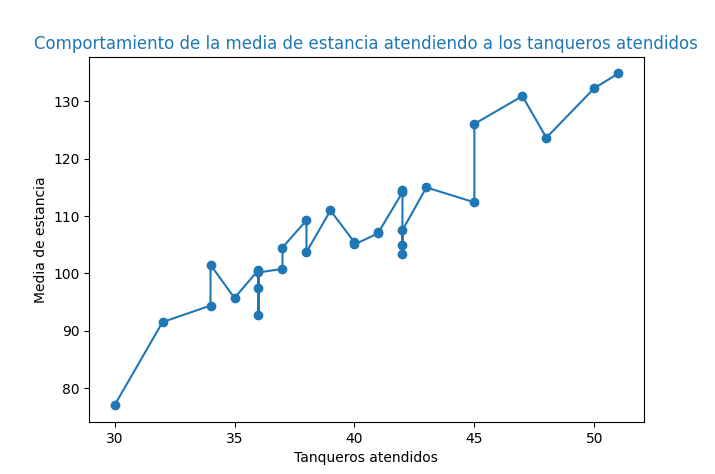
\includegraphics[scale=0.39]{img/Figure_2.png}
\caption{}

\end{figure}


Las gr\'aficas indican que los datos tienen una correlaci\'on lineal positiva, lo cual quiere decir que mientras el sistema permita la entrada de m\'as tanqueros, hay una tendencia a que m\'as tiempo se demore en terminar de atenderlos a todos y la media de estancia en el puerto sea mayor.

Por otro lado en $5$ horas que se permiti\'o la entrada de tanqueros al puerto se atendieron entre $30$ y $55$ barcos aproximadamente, esta diferencia viene dada por los diferentes tama\~nos que pueden tener los tanqueros, que influye en el tiempo de carga, adem\'as del tiempo de traslado hacia y desde los muelles, que puede demorarse en dependencia del tiempo generado por la distribuci\'on corresponiente. L\'ogicamente, si aumentamos las horas de entrada al puerto, entrar\'an m\'as tanqueros y el sistema se demorar\'a m\'as en atenderlos a todos; y la media de espera de los barcos ser\'a mayor. Esto se muestra en las gr\'aficas de la figura 2, donde se permiti\'o la entrada de tanqueros hasta $10$ horas.

\begin{figure}[h]

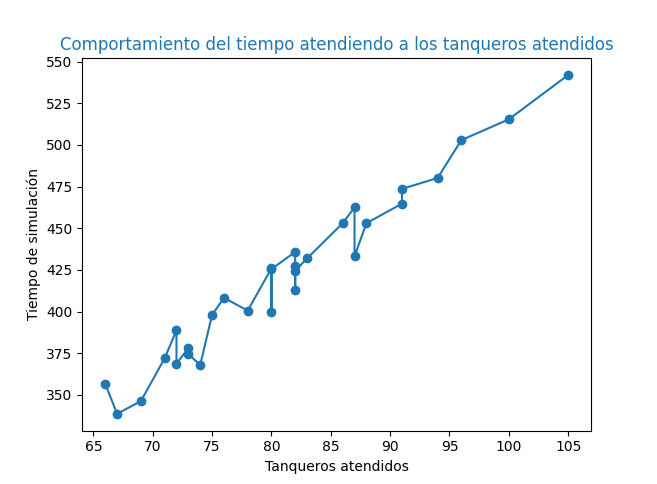
\includegraphics[scale = 0.39]{img/Figure_3.png}
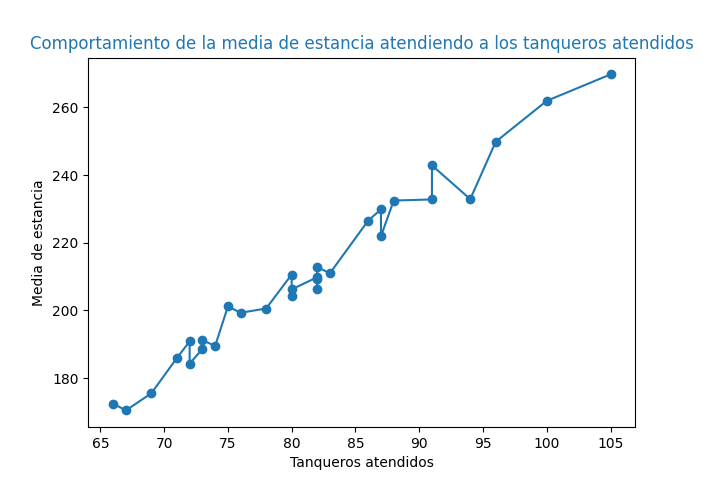
\includegraphics[scale=0.39]{img/Figure_4.png}
\caption{}

\end{figure} 

Podemos notar que entraron entre $65$ y $105$ barcos y que el tiempo de simulaci\'on y la media de estancia son mayores con respecto a las gr\'aficas de la figura 1.\\

Analicemos qu\'e ocurre si aumentamos el n\'umero de muelles que pueden atender tanqueros (el n\'umero de servidores aumenta). Las gr\'aficas siguientes corresponden a $30$ simulaciones permitiendo la entrada de barcos hasta $10$ horas en un puerto de $6$ muelles.\\


\begin{figure}[h]

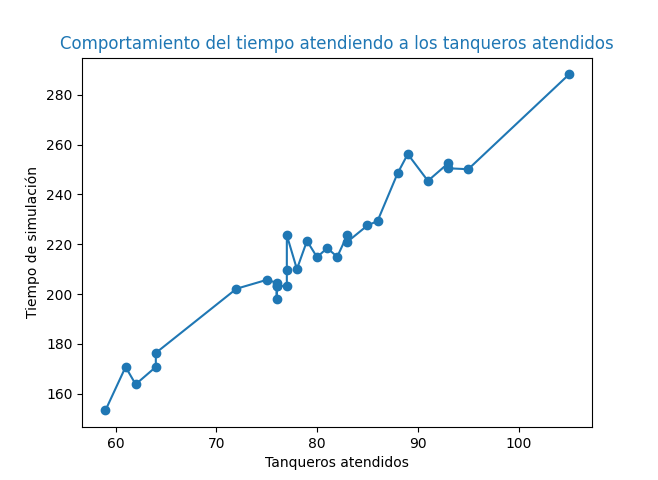
\includegraphics[scale = 0.39]{img/Figure_5.png}
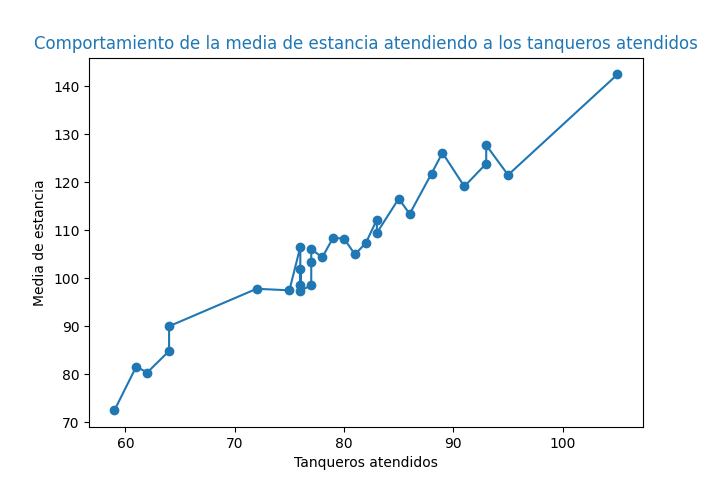
\includegraphics[scale=0.39]{img/Figure_6.png}
\caption{}

\end{figure} 

Comparando estos resultados con los de la figura 2, podemos llegar a la conclusi\'on de que, si aumenta el n\'umero de muelles, tanto el tiempo de simulaci\'on como la media de estancia disminuyen considerablemente. Ya que manteniendo los datos constantes y duplicando el n\'umero de muelles notamos que el tiempo de simulaci\'on pasa de entre las $350$ y $550$ horas a estar entre las $160$ y $280$ horas, tal como indican las gr\'aficas. De igual manera se nota una disminuci\'on de la estancia de las naves en el puerto de unas $120$ horas aproximadamente como promedio.\\\\

\section{Github}
En este \href{https://github.com/Alexx-4/Overloaded-Harbor.git}{\textcolor{red}{\underline{enlace}}} podemos encontrar el repositorio del proyecto en Github.



\end{document}